% Section 2.3 -- drop this in place of the three [TEAM MEMBER: ...] placeholders.
% Two things to fill in before submitting, both marked FILL below:
%   1. the exact final P&L (written here as roughly -$2,100)
%   2. the order your eliminations arrived in (the table is commented out;
%      uncomment it and fill the rows if you remember the order)
% The $0.15 minimum edge below is the default in the helper page; change it
% if you ran with a different number.
% Figure: upload ps2/figures/gtt_ladder.png to the Overleaf project (into a
% figures/ folder, or change the \includegraphics path). Needs \usepackage{graphicx},
% which the document almost certainly already has for Figures 1 and 2.

\subsection{Hashim Almodamagha}

\paragraph{Strategy going in.}
I went in planning to trade the gap between my private valuation and the market.
The private valuation was the equal-weight mean of the surviving set, $FV = \overline{S}$,
updated as each elimination printed, and the $\$0.02$ fee set the hurdle: I would buy
only when $FV - \text{ask}$ cleared the fee with room to spare and sell only when
$\text{bid} - FV$ did.

Size was to come from two inputs. The first was the deviation of the market price from
$FV$: the wider the gap, the larger the trade, since a wider gap is both more edge per
share and more room for the fee. The second was my remaining uncertainty over the
settlement value, which fell with every elimination: with five states alive a $\$1$ gap
between price and $FV$ is easily within the noise of my own estimate, but with two alive
it is a strong statement. So the rule was to scale size up in the deviation and down in
the uncertainty, trading small early when the surviving set was wide and committing
more as each news release narrowed it.

To run this without doing arithmetic under time pressure I built a small browser page
before the session (Figure~\ref{fig:ladder}): a vertical price ladder with the five
outcomes as rungs, where a click struck a value out as each elimination arrived. From the values still alive it
recomputed, under a uniform prior, the $FV$, the standard deviation I was sizing on
($\$2.83$ with all five alive, falling with each strike), and four prices drawn as
lines on the ladder: the buy and sell levels that cleared the fee plus a minimum edge,
and the risk-free bounds just outside the alive range, where any fill is profitable in
every state left. Entering the current quote returned a one-word signal, buy, sell,
hold or risk-free, with the edge per share after the fee, so each news release was a
click and a glance. The page could also fold my read of the market into the valuation,
marking a value as eliminated by the tape rather than by my news, and it flagged any
price that sat away from my $FV$ as a sign that other traders held eliminations I did
not. I had built that step and left it switched off.

\begin{figure}[htbp]
  \centering
  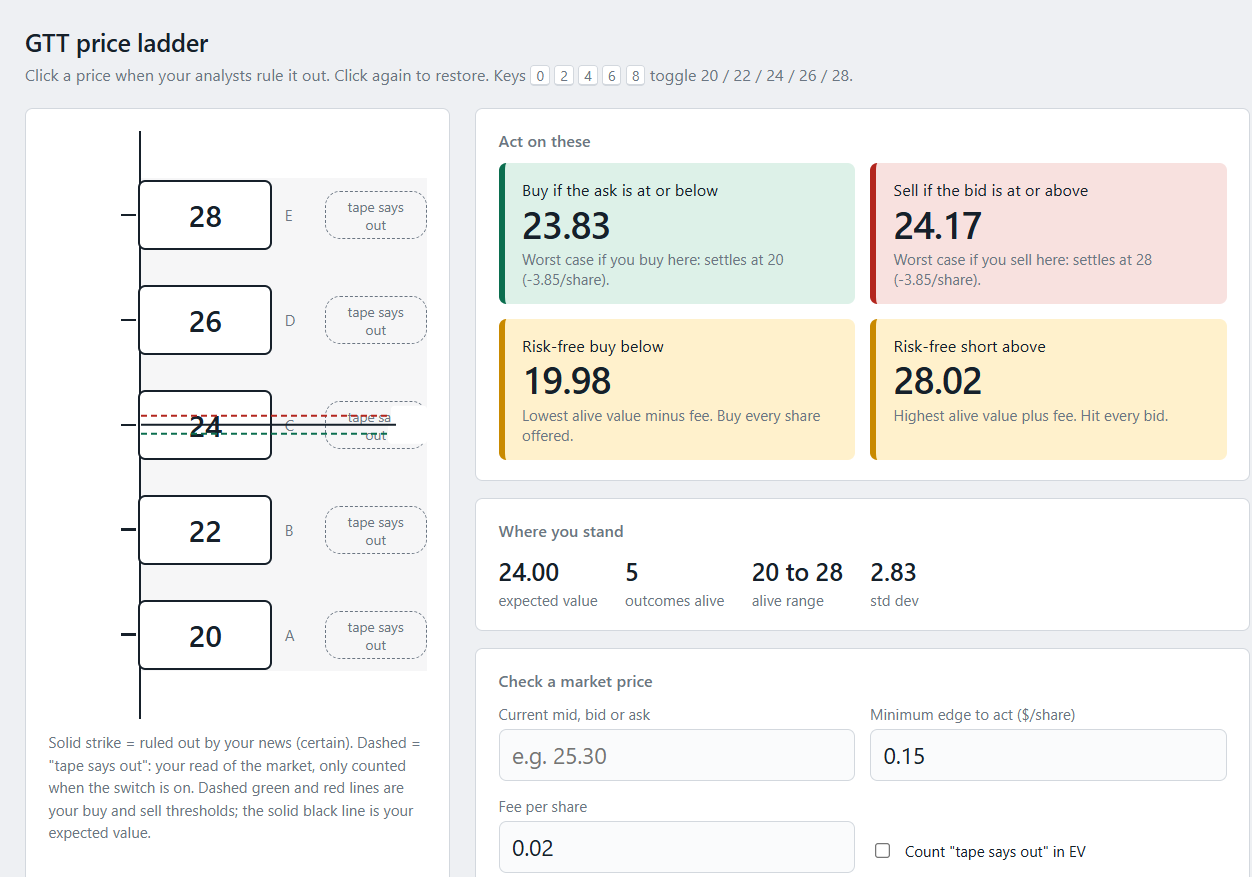
\includegraphics[width=\textwidth]{figures/gtt_ladder.png}
  \caption{The price ladder at the open, before any elimination. All five outcomes are
  alive, so the expected value is \$24.00 with a standard deviation of \$2.83. The
  dashed red and green lines on the ladder are the sell and buy thresholds (\$24.17 and
  \$23.83: expected value plus or minus the \$0.02 fee and a \$0.15 minimum edge), and
  the amber tiles are the risk-free bounds just outside the alive range. Striking a
  rung recomputes everything from the values left.}
  \label{fig:ladder}
\end{figure}

The premise was that eliminations would push the price around, that my own
eliminations would sometimes arrive before the market had absorbed the same
information, and that those moments would be the mispricings to trade. I had no plan
for what to do if the price simply did not move.

\paragraph{What happened.}
The price did not move. Through every elimination the market stayed pinned near $\$24$,
which was the unconditional mean at the open and turned out to be the settlement value.
Each elimination moved my own $FV$ off $\$24$, and I traded toward $FV$ because that
was the rule, but the market never followed. In hindsight, that was the case working as designed: each trader's surviving
set contains the truth, so the sets intersect only at the true value, and with
eliminations spread across the room the pressure from valuations above and below
$\$24$ cancelled. A price that refuses to leave $\$24$ while my $FV$ wanders away from
it is not a mispricing; it is the aggregate of everyone else's signals, and it was the
better estimate at every stage.
% \begin{center}
% \begin{tabular}{lccc}
% \toprule
% Stage & Surviving set $S$ & $FV=\overline{S}$ & Std.\ dev. \\
% \midrule
% Start           & $\{20,22,24,26,28\}$ & \$24.00 & 2.83 \\
% \$FILL eliminated & $\{\dots\}$          & \$FILL  & FILL \\
% \$FILL eliminated & $\{\dots\}$          & \$FILL  & FILL \\
% \$FILL eliminated & $\{\dots\}$          & \$FILL  & FILL \\
% \bottomrule
% \end{tabular}
% \end{center}

My own page was telling me this the whole time: every price I checked away from my
$FV$ came back with the warning that other traders probably held eliminations I did
not. I acted on the signal and ignored the warning. The risk-free bounds never came
into play either. The market never printed outside the alive range, for the same
reason it never left $\$24$: a price outside every trader's surviving set would have
required someone to sell below a value they knew was possible, and nobody did.

The consequence was that there was no edge of the kind I had prepared for, and the
sizing rule made it worse rather than better. Both of its inputs pointed the same way as
the round went on: each elimination widened the gap between the fixed price and my
moving $FV$ and at the same time shrank my uncertainty, so the rule
called for larger trades precisely when the market was telling me most clearly that my
$FV$ was the one that was wrong. Every position I took against the $\$24$ level was
marked back to $\$24$ at settlement, and every share paid the two-cent fee on the way
in. Net, I spent the round paying fees and spread to express a view the market had
already priced out.

\paragraph{P\&L and lessons.}
Final P\&L: roughly $-\$2{,}100$. % FILL: exact figure

Three things I would change. First, the valuation. The equal-weight mean of my own
surviving set is the right prior and the wrong posterior once the price is also an
observation. Next time a price that will not move toward my $FV$ gets treated as an
elimination I did not receive rather than as an opportunity, and the tool conditions
on it from the first tick.

Second, the shape of the strategy. Most of the round is news-free, and in those
stretches the only reliable income is the spread. I would conservatively make markets
around the prevailing price in the quiet periods, then, as a news release approached,
flatten inventory and wait rather than carry a position through the announcement.
Right after the release I would look for a genuine statistical arbitrage, a price
outside the range of my surviving set or a stale quote that has not caught up, where
the trade is profitable in every state I still consider possible. If none appeared I
would go back to making markets. That
keeps the directional risk confined to the moments when private information is actually
worth something, instead of running it all round.

Third, the objective. Looking at how the rest of the class finished, simply ending
above zero would have ranked well. The payoff structure of this case is asymmetric: the
gain from being right about a mispricing is a few cents per share, while the cost of
being confidently wrong is measured in dollars per share. Given that, I would prioritise
not losing over winning, trading smaller size, requiring a wider margin over the fee
before taking a statistical-arbitrage trade, and treating market making as the baseline
rather than as a fallback.
